% !LW recipe=uplatex
\documentclass[12pt,dvipdfmx]{article}
\usepackage[margin=1.0truein]{geometry}
\usepackage{ifdraft}
\usepackage{subfiles}

% Math
\usepackage{amsmath}
\usepackage{amssymb}
\usepackage{bm}
\usepackage{mathrsfs}
\usepackage{mathtools}
\usepackage{optidef}
\usepackage{physics}
% https://qiita.com/rityo_masu/items/efd44bc8f9229e014237
\allowdisplaybreaks[4]
\DeclarePairedDelimiter{\floor}{\lfloor}{\rfloor}
\DeclarePairedDelimiter{\ceil}{\lceil}{\rceil}
% https://tex.stackexchange.com/questions/28836/typesetting-the-define-equals-symbol
% https://tex.stackexchange.com/questions/5502/how-to-get-a-mid-binary-relation-that-grows
\newcommand{\relmiddle}[1]{\mathrel{}\middle#1\mathrel{}}

% Theorem environments
\usepackage{amsthm}
\usepackage{thm-restate}
\theoremstyle{plain}
\newtheorem{theorem}{Theorem}
\newtheorem{proposition}{Proposition}
\newtheorem{lemma}{Lemma}
\newtheorem{assumption}{Assumption}
\newtheorem{condition}{Condition}
\newtheorem{corollary}{Corollary}

% Figure, Table, Algorithm
\usepackage{graphicx}
\usepackage{booktabs}
\usepackage{multirow}
\usepackage{makecell}
% \usepackage{mathptmx}
\usepackage{subcaption}
\usepackage{float}
\usepackage{tikz}
\definecolor{cA}{HTML}{0072BD}
\definecolor{cB}{HTML}{EDB120}
\definecolor{cC}{HTML}{77AC30}
\definecolor{cD}{HTML}{D95319}
\newcommand{\red}[1]{\textcolor{red}{#1}}
\newcommand{\blue}[1]{\textcolor{blue}{#1}}
\newcommand{\cyan}[1]{\textcolor{cyan}{#1}}
\newcommand{\gray}[1]{\textcolor{gray}{#1}}
\newcommand{\green}[1]{\textcolor{green}{#1}}
\newcommand{\brown}[1]{\textcolor{brown}{#1}}
\newcommand{\black}[1]{\textcolor{black}{#1}}
\newcommand{\orange}[1]{\textcolor{orange}{#1}}

% References
\usepackage{hyperref}
\usepackage{cleveref}
% cleveref fails to accurately capture pseudo-code line numbers. We define a custom reference command for lines in algorithms.
\crefname{assumption}{Assumption}{Assumptions}
\newcommand{\refLine}[1]{Line~\ref{#1}}
\newcommand{\refLines}[2]{Lines~\ref{#1} and \ref{#2}}

% Other packages
\usepackage{appendix}
\usepackage{cancel}
\usepackage{enumitem}
\usepackage{fancybox}
\usepackage{ifthen}
\usepackage{lipsum}
\usepackage{pifont}
\usepackage{xparse}

% https://www.reddit.com/r/LaTeX/comments/111e7gn/can_someone_help_me_replicate_these_boxes_in_latex/
\usepackage{tcolorbox}
\tcbuselibrary{skins, breakable}
\NewTotalTColorBox[auto counter]{\bookBox}{ +m +m }{
    notitle,
    colback=white,
    frame hidden,
    boxrule=0pt,
    enhanced,
    sharp corners,
    borderline west={4pt}{0pt}{cA},
    breakable,
}{
    \textcolor{cA}{
        \sffamily\textbf{#1}
    }#2
}
\NewTotalTColorBox[auto counter]{\myBox}{ +m +m }{
    notitle,
    colback=white,
    frame hidden,
    boxrule=0pt,
    enhanced,
    sharp corners,
    borderline west={4pt}{0pt}{cC},
    breakable,
}{
    \textcolor{cC}{
        \sffamily\textbf{#1}
    }#2
}

\begin{document}

\title{Supplemental Material for 06/30\\Book Reading Seminar}
\author{Hiroki Hamaguchi}
\date{2026/06/30}
\maketitle

\begin{abstract}
    \begin{center}
        This is the supplemental material for the book reading seminar.

        If necessary, please also refer to my \href{https://github.com/hari64boli64/BookReadingSeminarMaterials}{repository}.

        The textbook link of Springer is \href{https://link.springer.com/book/10.1007/b97543}{here}.
    \end{center}
\end{abstract}

\myBox{Chapter1からの復習事項}{\\
    変分不等式 (Variational Inequality) $\operatorname{VI}(K,F)$:
    \begin{equation*}
        \text{Find} \quad x \in K \quad \text{s.t.} \quad (y-x)^\top F(x) \geq 0 \quad \text{for all} \quad y \in K.
    \end{equation*}
    (本稿で繰り返し現れる解釈: \href{https://www.kurims.kyoto-u.ac.jp/coss/coss2019/hayashi-lecture1.pdf}{林先生の資料} p.16 「変分不等式問題は集合 $K$ 上で働く力のベクトル場 $-F$ に対する『安定点』を求める問題」)\\
    線形相補性問題 (Linear Complementarity Problem) $\operatorname{LCP}(q,M)$:
    \begin{equation*}
        \text{Find} \quad x \in \mathbb{R}^n \quad \text{s.t.} \quad 0 \leq x \perp Mx+q \geq 0.
    \end{equation*}
    (LCPはVIの特殊形: \href{https://www.kurims.kyoto-u.ac.jp/coss/coss2019/hayashi-lecture1.pdf}{林先生の資料} p.21)
}

\bookBox{P.419 第1段落}{
    $\operatorname{VI}(K,F)$ の解が、集合 $K$ や写像 $F$ の小さな変化に対してどのように変化するかを調べる。
    厳密には、閉凸集合の族および連続写像の空間に距離を導入して「小さな変化」を定式化する必要がある。
}

\bookBox{P.419 第2段落}{
    孤立解 $x^*$ を一つ固定し、摂動後の問題 $\operatorname{VI}(L,G)$ に $x^*$ の近くの解が存在するか、その解が孤立しているか、摂動が消えるとき近傍の解が $x^*$ に収束するかを問うのが\textbf{孤立感度解析 (isolated sensitivity analysis)}である。
}

\bookBox{P.419 第3段落、P.420 第2段落}{
    パラメータ付き問題
    \[
        \{\operatorname{VI}(K(p),F(\cdot,p)) : p\in P\}
    \]
    では、$p^*$ における解 $x^*$ から出る解軌道 $x(p)$ の連続性に加え、微分可能性も問題となる。
    このような問題は\textbf{孤立パラメトリック解析 (isolated parametric analysis)}と呼ばれる。
    とくに本章前半では $K$ を固定し $F$ のみを摂動する。この設定は MiCP や NCP の感度解析を含む。
}

\bookBox{P.420 第3段落}{
    解集合全体 $\operatorname{SOL}(K,F)$ の変化を調べるのが\textbf{全感度解析}である。
    こちらの方が一般に難しく、あまり扱わない。
}

\myBox{最適化問題との対応}{
    $F=\nabla f$ のとき、$\operatorname{VI}(K,F)$ は制約付き最適化の一階条件である。
    したがって孤立感度解析は、目的関数やパラメータを少し変えた際に局所解が残るか、また解がどの程度動くかを調べる問題と解釈できる(cf.\ LPの感度分析)。
    ただし一般の VI ではポテンシャル $f$ が存在するとは限らず、あくまで直感的理解の補助。
}

\bookBox{Example 5.1.1}{\\
    $K$: 固定された閉凸集合\qquad
    $x^*$: $\operatorname{VI}(K,F)$ の局所一意解\\

    ナイーブな予想「$G \approx F$ に対して $\operatorname{VI}(K,G)$ が $x^*$ の近くに解をもつ」\\
    しかし局所一意性だけではこれを保証できない。
    反例が例5.1.1。
    \[
        q=(0,-1,1)^\top,\qquad
        M=\begin{bmatrix}0&-1&-1\\1&0&0\\-1&0&0\end{bmatrix}
    \]
    による LCP は一意解 $(1,0,0)$ をもつ一方、$q(\varepsilon)=(\varepsilon,-1,1)^\top$
    とすると任意の $\varepsilon<0$ で解が存在しない。
    この例外をどう説明するか?
    また、この反例より「元の解($x^*_F \in \operatorname{SOL}(K,F)$)が孤立していること」と「近い問題($\operatorname{SOL}(K,G \approx F)$)に近い解($x^*_G \approx x^*_F$)が存在すること」は別の性質だと分かる。

    \begin{figure}[H]
        \centering
        \includegraphics[width=0.75\columnwidth]{example5.1.1.png}
    \end{figure}
}

\myBox{関数の近傍の定義}{
    開集合 $D\subseteq\mathbb R^n$ 上の連続写像 $H$ と $S\subset D$ に対し、
    \[
        \mathbb B(H;\varepsilon,S)
        \coloneqq\left\{G:\sup_{y\in S}\norm{G(y)-H(y)}<\varepsilon\right\}
    \]
    を $S$ 上の一様な $\varepsilon$-近傍とする。$\norm{G_k-H}_S \coloneqq \sup_{y \in  S} \norm{G(y)-H(y)} \to 0$ を $G_k$ が $S$ 上で $H$ に収束することと呼ぶ。(一様収束に近い定義)
}

\bookBox{命題5.1.2:孤立解は近傍解の集積点である}{
    $F\colon D\to\mathbb R^n$ を連続とし、$x^*$ を $\operatorname{VI}(K,F)$ の孤立解とする。
    $x^*$ の近傍 $N$ が
    \[
        \overline N\subset D,\qquad
        \operatorname{SOL}(K,F)\cap\overline N=\{x^*\}                         \tag{5.1.1}
    \]
    を満たすとする。$G_k\to F$ が $N$ 上で一様に成り立ち (i.e., $\lim_{k \to \infty} \norm{G_k - F}_N=0$)、
    $x_k\in\operatorname{SOL}(K,G_k) \red{{} \cap N}$ ならば $x_k\to x^*$ である。

    \begin{figure}[H]
        \centering
        \includegraphics[width=0.75\columnwidth]{proposition5.1.2.png}
    \end{figure}

    証明の要点はコンパクト性と極限操作。
    $\{x_k\}$ の任意の集積点 $x^\infty$ は、$G_k\to F$ と VI の不等式を極限に移すことにより $\operatorname{VI}(K,F)$ の解となる。
    しかも $x^\infty\in\overline N$ なので (5.1.1) より $x^\infty=x^*$ である。
    集積点が一つしかないため列全体が $x^*$ に収束する。\\

    ただし、この命題は\red{摂動後の解が近傍に存在する}と仮定してその収束を述べる。
    存在そのものは保証しない。
    この``local solvability''を、degree theoryを用いて解析する。
}

\myBox{natural mapとnormal map}{\\
    natural map:
    \begin{equation*}
        F_K^{\mathrm{nat}}(v) \coloneqq v - \Pi_K(v-F(v)).
    \end{equation*}
    Proposition 1.5.8 ($K$: closed convex):
    \begin{equation*}
        x \in \operatorname{SOL}(K,F) \iff F_K^{\mathrm{nat}}(x) = 0
    \end{equation*}
    雑理解: VIは $-F$ の $K$ 上安定点を求める問題。natural mapは $-F$ 方向に進む射影勾配降下法の1ステップ。Prop. 1.5.8の証明はVIと $\Pi$ の定義より不等式評価。\\

    normal map:
    \begin{equation*}
        F_K^{\mathrm{nor}}(v) \coloneqq F(\Pi_K(v)) + v - \Pi_K(v).
    \end{equation*}
    Proposition 1.5.9 ($K$: closed convex):
    \begin{equation*}
        x \in \operatorname{SOL}(K,F) \iff \exists z \in \mathbb{R}^n \text{ s.t. } x=\Pi_K(z) \text{ and } F_K^{\mathrm{nor}}(z)=0
    \end{equation*}
    雑理解: normal mapの零点 $z$ は、射影した先の点 $x$ がVIの解であることを保証する、証明はVIと $\Pi$ の定義より不等式評価。

    \begin{figure}[H]
        \centering
        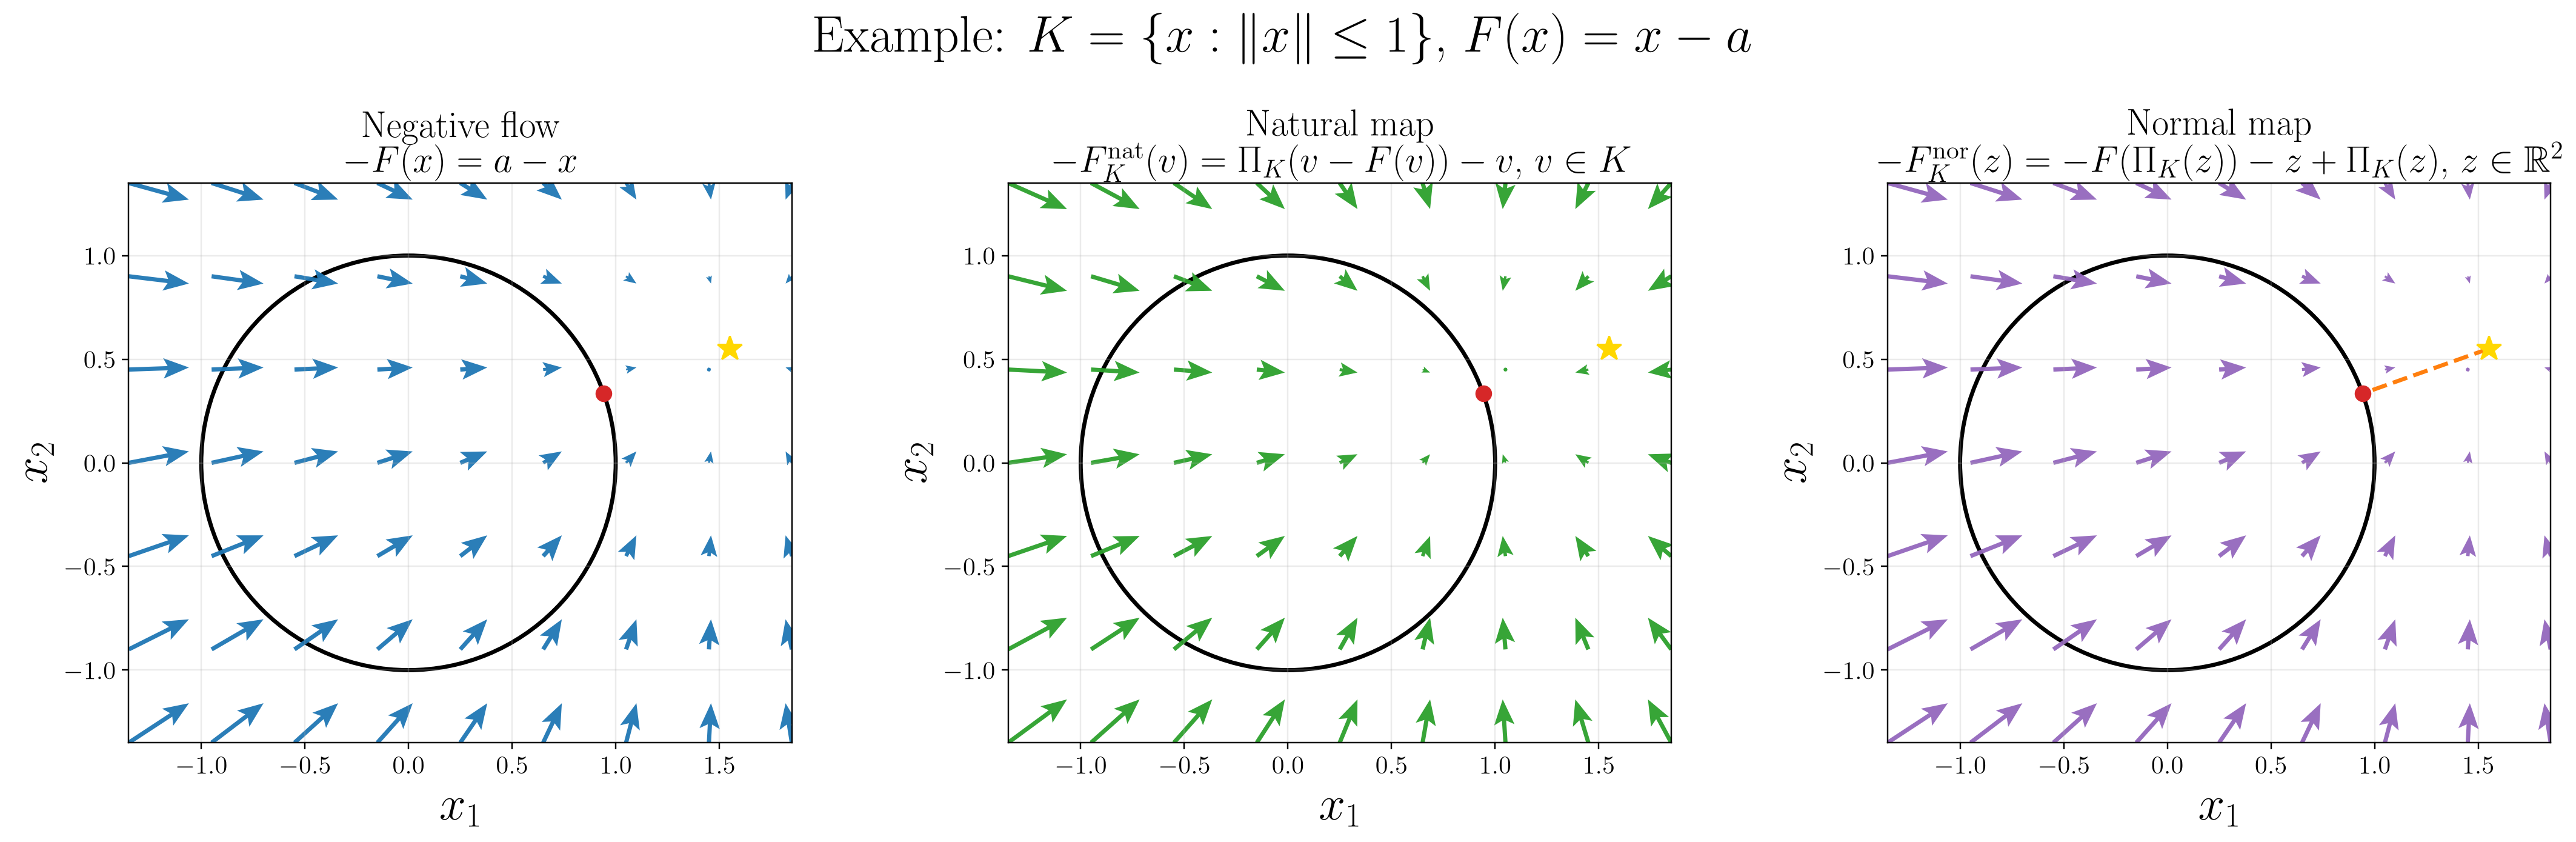
\includegraphics[width=\columnwidth]{nat_and_nor.png}
        \caption{natural mapとnormal mapの例}
    \end{figure}
    \textbf{直観としては、natural mapを使えば、安定性の定義に出てくるSOLという扱いにくい集合が、零点の問題に帰着できるので嬉しい。}
}

\myBox{degree theory}{
    (Definition 2.1.1、Proposition 2.1.3など)\\
    $\Omega\subset\mathbb R^n$ を有界開集合、$\Phi\colon\overline\Omega\to\mathbb R^n$
    を連続写像とし、$p\notin\Phi(\partial\Omega)$ とする。
    \[
        \deg(\Phi,\Omega,p)\in\mathbb Z
    \]
    は、大雑把には $\Omega$ 内にある方程式 $\Phi(x)=p$ の零点の向き付き個数を表す。
    $p=0$ のときは $\deg(\Phi,\Omega)\coloneqq\deg(\Phi,\Omega,0)$ と略記する。
    また、以下が成り立つ。
    \[
        p \notin \Phi(\operatorname{bd}(\Omega)) \; \mathrm{and} \;
        \deg(\Phi,\Omega,p)\ne0
        \implies
        \text{$\Phi(x)=p$ は $\Omega$ 内に解をもつ},
    \]
    $\bar x$ を $\Phi(x)=p$ の孤立解とする。
    $\bar x$ だけを含み、ほかの解を含まない十分小さな開近傍 $U$ をとると、$\deg(\Phi,U,p)$ は $U$ の選び方によらない。この共通値を
    \[
        \operatorname{ind}(\Phi,\bar x)
        \coloneqq \deg(\Phi,U,p)
    \]
    と定める。\\
    \textbf{直観としては、零点の問題に帰着したので、degree theoryで処理する、いつもの流れ。}
}

\myBox{境界など}{
    $\partial N$ は集合 $N$ の境界。
    また、
    \[
        \operatorname{dist}_\infty(0,\Phi(\partial N))
        =\inf_{x\in\partial N}\norm{\Phi(x)}_\infty
    \]
    は、境界上で $\Phi$ が零点からどれだけ離れているかを測る量である。
    一般に、閉集合 $S\subset\mathbb R^n$ に対して
    \[
        \operatorname{dist}_\infty(x,S)
        \coloneqq\inf_{y\in S}\norm{x-y}_\infty
    \]
    と定義される（後述参照）。
}

\myBox{Nearness Property}{
    \begin{figure}[H]
        \centering
        \includegraphics[width=\columnwidth]{nearness1.png}
    \end{figure}
    \begin{figure}[H]
        \centering
        \includegraphics[width=\columnwidth]{nearness2.png}
    \end{figure}
    ホモトピー変換の間で常に、境界上で零点が発生しないなら、degreeは不変 (公理A3)。
    \textbf{直観としては、関数値の変動幅の最大値が、もともとの境界上における零点からの最短距離で上からバウンドされているなら、常に境界上で零点が発生せず、degree不変。}
    \textcolor{gray}{
\begin{proof}
    \textcolor{gray}{
    Definition 2.1.1 の公理A3 はホモトピー不変性を主張する:
    \begin{equation*}
        H\colon\overline{\Omega}\times[0,1]\to\mathbb{R}^{n},
    \end{equation*}
    \begin{equation*}
        p \notin H(\partial\Omega,t) \implies         \deg(H(\cdot,t),\Omega,q(t)) \text{が不変}
    \end{equation*}
    }
    \textcolor{gray}{
    ここで、
    \begin{equation*}
        H(x,t)\coloneqq
        (1-t)\Phi(x)+t\Upsilon(x)
    \end{equation*}
    とし、 $x\in\partial\Omega$ および $t\in[0,1]$ に対して、
    \begin{align*}
        \|H(x,t)-p\|_{\infty}
        &=
        \|\Phi(x)-p+t(\Upsilon(x)-\Phi(x))\|_{\infty}
        && (\text{definition of $H$})\\
        &\geq
        \|\Phi(x)-p\|_{\infty}
        -t\|\Upsilon(x)-\Phi(x)\|_{\infty}
        &&(\text{triangle inequality})\\
        &\geq
        \operatorname{dist}_{\infty}
        \bigl(p,\Phi(\partial\Omega)\bigr)
        -\|\Upsilon(x)-\Phi(x)\|_{\infty}
        &&(\text{definition of $\mathrm{dist}$ and $t\leq 1$})\\
        &\geq
        \operatorname{dist}_{\infty}
        \bigl(p,\Phi(\partial\Omega)\bigr)
        -
        \max_{y\in\overline{\Omega}}
        \|\Phi(y)-\Upsilon(y)\|_{\infty}
        &&(\text{max})\\
        &>0 && (\text{assumption})
    \end{align*}
    より、$p\notin H(\partial\Omega,t)$ なので、$\deg(\Phi,\Omega,p)=\deg(\Upsilon,\Omega,p)$.
    }
\end{proof}}
}

\bookBox{命題5.1.3:natural mapによる局所可解性}{
    $F_K^{\mathrm{nat}}$ をnatural mapとする。孤立解 $x^*$ における \red{$\operatorname{ind}(F_K^{\mathrm{nat}},x^*)$ が非零}ならば、(5.1.1) を満たす任意の開近傍 $N$ に対し、
    \[
        \varepsilon=\operatorname{dist}_\infty
        (0,F_K^{\mathrm{nat}}(\partial N))>0
    \]
    とおくことで、$\norm{G-F}_{\overline N}<\varepsilon$ を満たす $G$ による
    $\operatorname{VI}(K,G)$ は $N$ 内に解をもつ。

    (直観としては自明、証明も難しくない、略)
}

\myBox{議論の流れの整理}{
    ここまでの議論で、
    \begin{itemize}
        \item 命題5.1.2 → 摂動問題でも解が非空かどうかが、感度分析の本質
        \item 命題5.1.3 → indの値が非零かどうかが、摂動問題でも解が非空かどうかかの本質
    \end{itemize}
    ということが分かった。
    このindの値が非零という条件を、もう少し扱いやすくしていくのが、命題5.1.4と系5.1.5。
}


\bookBox{命題5.1.4:normal mapによる誤差条件の局所化}{
    $F_K^{\mathrm{nor}}$ をnormal mapとし、$z^*=x^*-F(x^*)$ とする。孤立解 $x^*$ に対応する
    \red{$\operatorname{ind}(F_K^{\mathrm{nor}},z^*)$ が非零}ならば、(5.1.1) を満たす任意の開近傍 $N$ に対し、
    $\Pi_K(Z)\subset N$ かつ $z^*$ が $\overline Z$ における $F_K^{\mathrm{nor}}$ の唯一の零点となる
    $z^*$ の開近傍 $Z$ をとり、
    \[
        \varepsilon=\operatorname{dist}_\infty
        (0,F_K^{\mathrm{nor}}(\partial Z))>0
    \]
    とおくことで、$K_N=K\cap\overline N$ 上で
    $\norm{G-F}_{K_N}<\varepsilon$ を満たす $G$ による
    $\operatorname{VI}(K,G)$ は $N$ 内に解をもつ。

    この命題は、natural mapの場合に比べ、関数の変動をバウンドすべき領域が $K_N = K \cap \overline{N}$ という、より小さい範囲に限定されている(ただし、$\epsilon$ も変わっているので、完全上位互換という訳ではない)。
    その理由は、proofにもある不等式の行間を埋めれば分かる:
    \begin{align*}
        &\sup_{z \in \operatorname{cl} \mathcal{Z}} \norm{G_K^{\mathrm{nor}}(z)-F_K^{\mathrm{nor}}(z)} && (\text{左辺})\\
        ={}&\sup_{z \in \operatorname{cl} \mathcal{Z}} \norm{G(\Pi_K(z))+z-\Pi_K(z)-F(\Pi_K(z))-z+\Pi_K(z)} && (\text{normal mapの定義})\\
        \leq{} & \sup_{z \in \operatorname{cl} \mathcal{Z}} \norm{G(\Pi_K(z))-F(\Pi_K(z))} && (\text{整理})\\
        \leq {}& \sup_{x \in K \cap \operatorname{cl} \mathcal{N}} \norm{G(x)-F(x)}_2 && (\text{射影の定義})\\
        < {}& \epsilon. &&(\text{右辺})
    \end{align*}
}

\bookBox{系5.1.5:パラメータ付きVIの局所可解性と収束 \red{($H$ は $F$ の誤植!)}}{
    パラメータ付きの固定集合 VI では、$F(\cdot,p^*)$ に対するnormal mapの指数が非零で、
    \[
        \sup_{x\in K\cap N}\norm{F(x,p)-F(x,p^*)}
        \le L\norm{p-p^*}
    \]
    が成り立つなら、$p^*$ の十分小さい近傍で
    $S_N(p)=\operatorname{SOL}(K,F(\cdot,p))\cap N$ は空でない。さらに
    \[
        \lim_{p\to p^*}\sup\{\norm{x-x^*}:x\in S_N(p)\}=0.                 \tag{5.1.3}
    \]

    これはかなり自明。リプシッツ連続性から、命題5.1.4の条件にある関数の変動幅の条件 ($\norm{G-F}_{K_N}<\epsilon$) を十分近傍に取れば満たせるので、前半は直ちに従う。
    後半も、解があることが既に分かっているので、命題5.1.2 (孤立解は近傍解の集積点である) より、解は集積するので、式(5.1.3)も自明。
}

\myBox{具体例による確認}{
    結局、これまでの話は、indの値が非零というのが非常に強い条件であるということに基づいていた。そもそも、このindの値が非零とはどういうことを意味していたか?

    Example 5.1.1と同じ現象は2次元でも確認できる。$K=\mathbb{R}_+^2$ とし、
    \[
        F_\varepsilon(x)=
        \begin{bmatrix}x_1-1\\-x_2-\varepsilon\end{bmatrix},
        \qquad
        q_\varepsilon=\begin{bmatrix}-1\\-\varepsilon\end{bmatrix},
        \qquad
        M=\begin{bmatrix}1&0\\0&-1\end{bmatrix}
    \]
    によるLCPを考える。

    \begin{figure}[H]
        \centering
        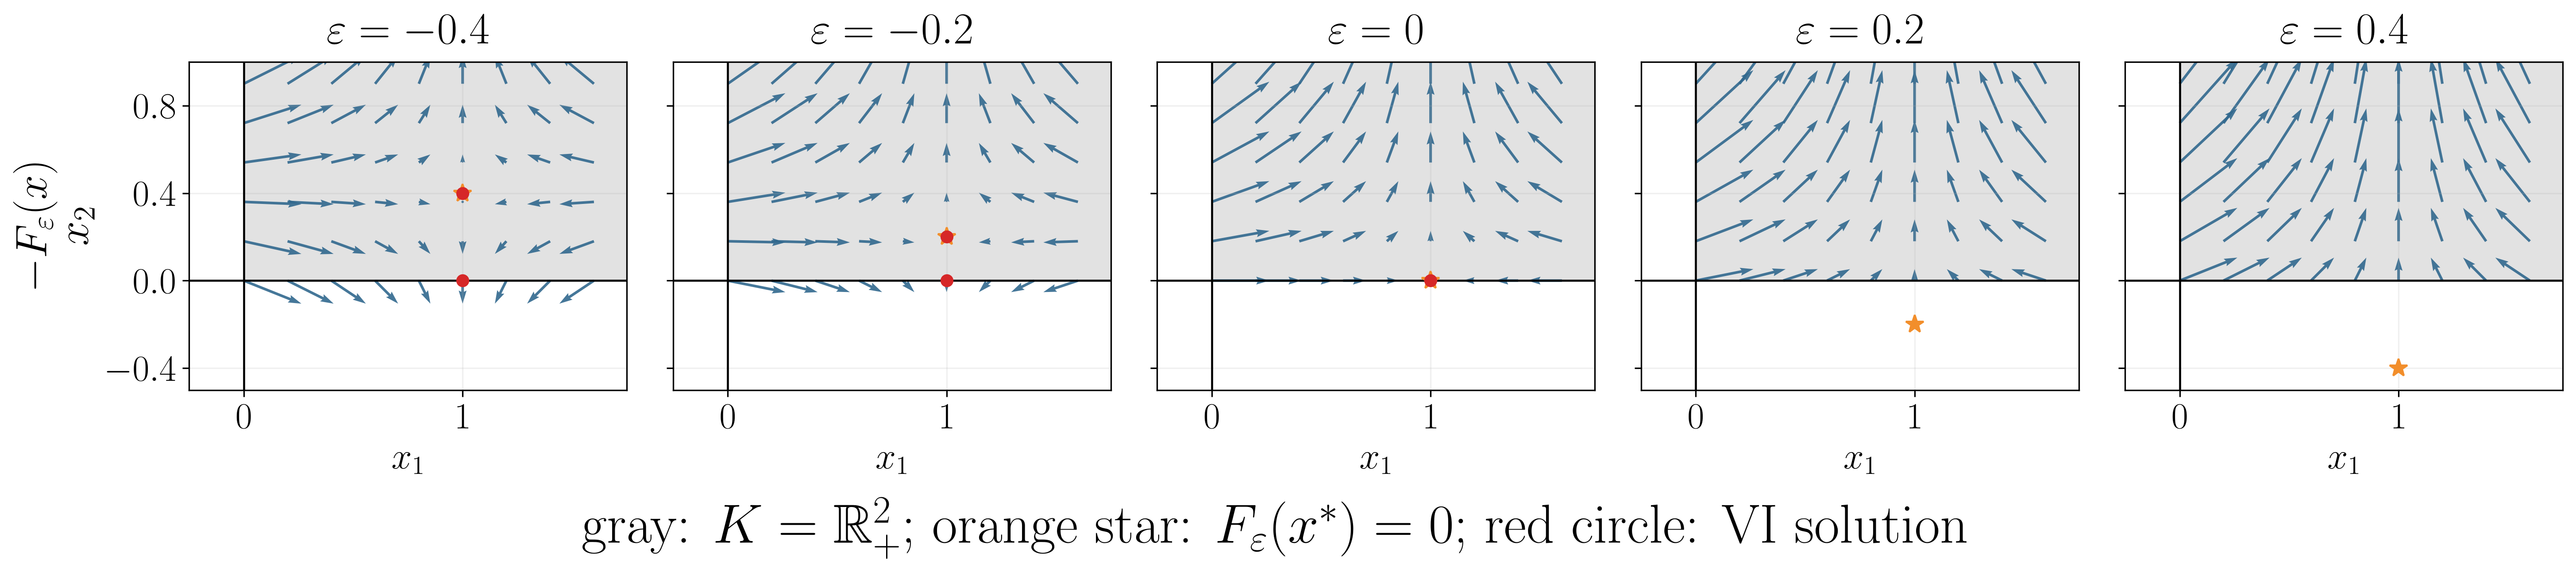
\includegraphics[width=\columnwidth]{index_zero_example.png}
        \caption{$-F_\varepsilon$ の変化。灰色の領域は
        $K=\mathbb{R}_+^2$、橙色の星は $F_\varepsilon$ の零点、赤丸はVIの解を表す。
        $\varepsilon<0$ の2つの解が
        $\varepsilon=0$ で合流し、$\varepsilon>0$ で消滅する。}
    \end{figure}

    \begin{figure}[H]
        \centering
        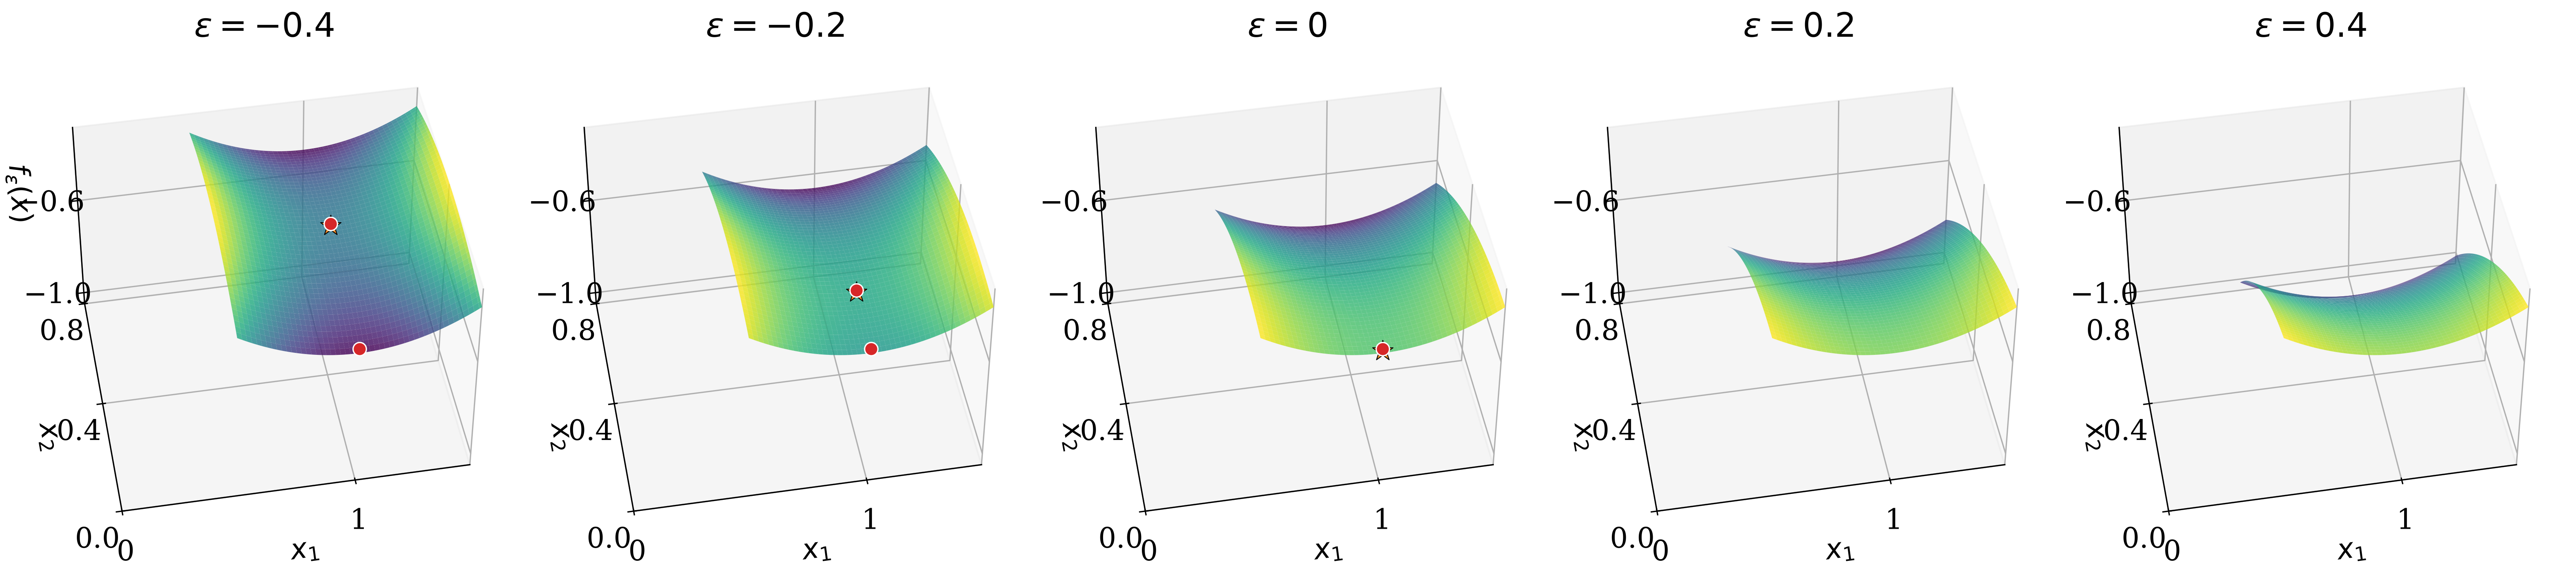
\includegraphics[width=\columnwidth]{optimization_surface_example.png}
        \caption{quiverで示した矢印が、$-\nabla f$ となるような $f$ のプロット。最適化で言う鞍点に $x^*$ があるとマズいということを主張している。完全に鞍点と1対1対応している訳ではないので注意が必要だが、理解には役立つ。}
    \end{figure}


    この消滅をindから確認しよう。射影を成分ごとに計算すると
    \[
        (F_0)_K^{\mathrm{nat}}(x)
        =x-\Pi_K(x-F_0(x))
        =\begin{bmatrix}x_1-1\\-|x_2|\end{bmatrix}.
    \]
    \begin{figure}[H]
        \centering
        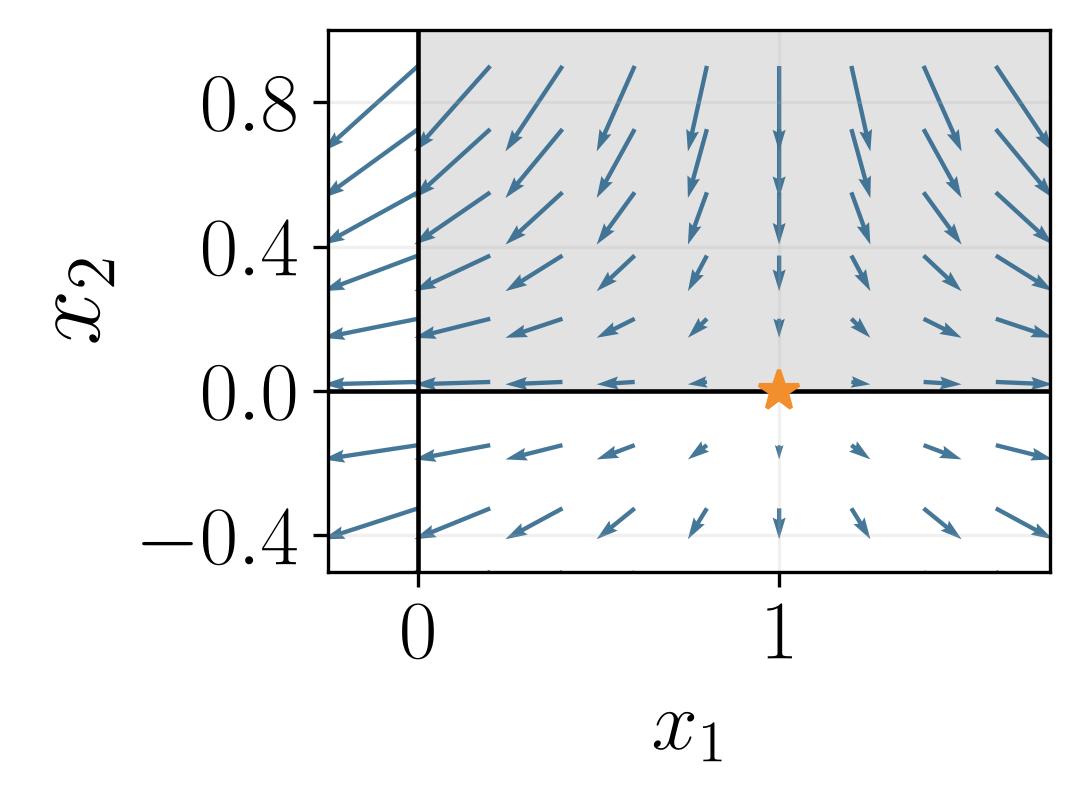
\includegraphics[width=0.4\columnwidth]{absolute_value_vector_field.png}
        \caption{$(F_0)_K^{\mathrm{nat}}(x)$}
    \end{figure}

    \begin{figure}[H]
        \centering
        \fbox{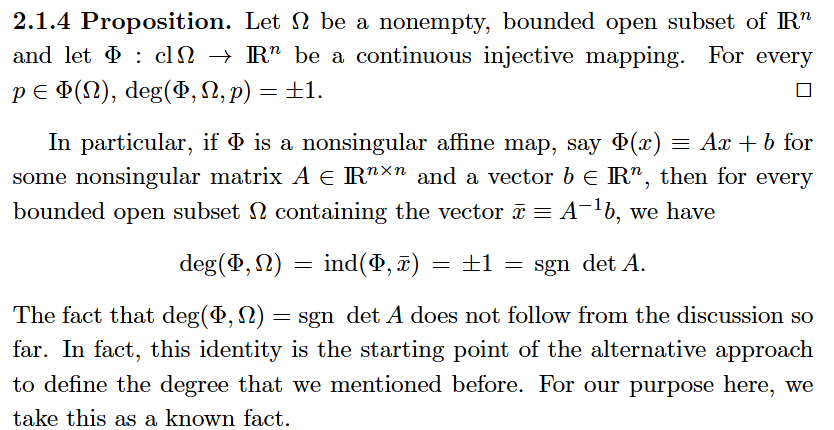
\includegraphics[width=\columnwidth]{prop2.1.4.png}}
    \end{figure}

    $u=x_1-1$, $v=x_2$ とおき、原点に十分近い正則値
    $p=(a,-b)$（$b>0$）をとると、その逆像は $(a,b)$ と $(a,-b)$ の2点である。
    $v>0$ では写像は $(u,v)\mapsto(u,-v)$ で行列式の符号は $-1$、
    $v<0$ では $(u,v)\mapsto(u,v)$ で行列式の符号は $+1$ である。したがって
    Proposition 2.1.3~(g) の領域分割に関する加法性と、Proposition 2.1.6 の
    逆像点ごとのindexの加法性を用いると、
    \[
        \operatorname{ind}((F_0)_K^{\mathrm{nat}},x^*)
        =(-1)+(+1)=0.
    \]
    正確には「領域自体のindex」を足すのではなく、正則値の各逆像を互いに素な
    近傍で囲み、各近傍の次数 $\operatorname{sgn}\det A$ を足している。
}

\myBox{議論の流れの整理}{
    ここまでの議論で、(リプシッツ性の仮定のもとで)
    \begin{itemize}
        \item 命題5.1.2 → 摂動問題でも解が非空かどうかが、感度分析の本質
        \item 系5.1.4 → indの値が非零かどうかが、摂動問題でも解が非空かどうかかの本質
    \end{itemize}
    ということが分かった。そして、
    \begin{itemize}
        \item 以降の議論 → 臨界錐上の正値性が、indの値が非零かどうかの本質
    \end{itemize}
    という議論を展開する。
}

\myBox{臨界錐}{
    \begin{figure}[H]
        \centering
        \fbox{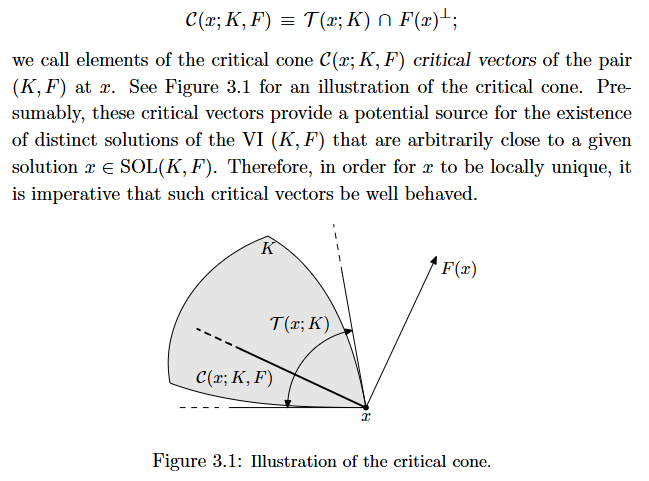
\includegraphics[width=\columnwidth]{critical_cone.png}}
    \end{figure}
}

\bookBox{命題5.1.6:臨界錐上の正値性}{
    $F$ が解 $x^*$ で B微分可能とする。臨界錐
    \[
        \mathcal{C}(x^*;K,F)=\mathcal{T}(x^*;K)\cap F(x^*)^\perp
    \]
    上で
    \[
        v^\top F'(x^*;v)>0
        \qquad(0\ne v\in C(x^*;K,F))                                  \tag{5.1.4}
    \]
    が成り立つなら、natural mapとnormal mapの指数はいずれも定義され非零となる。
}

\myBox{具体例による確認}{
    先ほどの例では $F_0(x^*)=0$ なので、critical cone は
    \[
        \mathcal{C}(x^*;K,F_0)
        =\mathcal{T}(x^*;K)\cap F_0(x^*)^\perp
        =\mathbb{R}\times\mathbb{R}_+.
    \]
    特に $v=(0,1)^\top$ に対して
    $v^\top F_0'(x^*;v)=-1<0$ であり、命題5.1.6の条件 である式(5.1.4) は成立しない。

    また、もし$F_0(x^*) \neq 0$の場合、critical coneは、
    \[
        \mathcal{C}(x^*;K,F_0)
        =\mathcal{T}(x^*;K)\cap F_0(x^*)^\perp
        =\mathbb{R}\times\{0\}.
    \]
    つまり、横方向の直線となる。
    式(5.1.4)の意味としては、横方向に少しだけ動いても、元の場所に戻る方向に力が働く ($v^\top (-F'(x^*;v))<0$) ということになる。
}

\myBox{二次十分条件との類似}{
    式(5.1.4) は、最適化において臨界方向上で曲率が正であるという二次十分条件に対応する形をしている。
    $F=\nabla f$ が滑らかなら $F'(x^*;v)=\nabla^2f(x^*)v$ なので、左辺は
    $v^\top\nabla^2f(x^*)v$ となる。この正値性が局所一意性などを与えている。

    \begin{figure}[H]
        \centering
        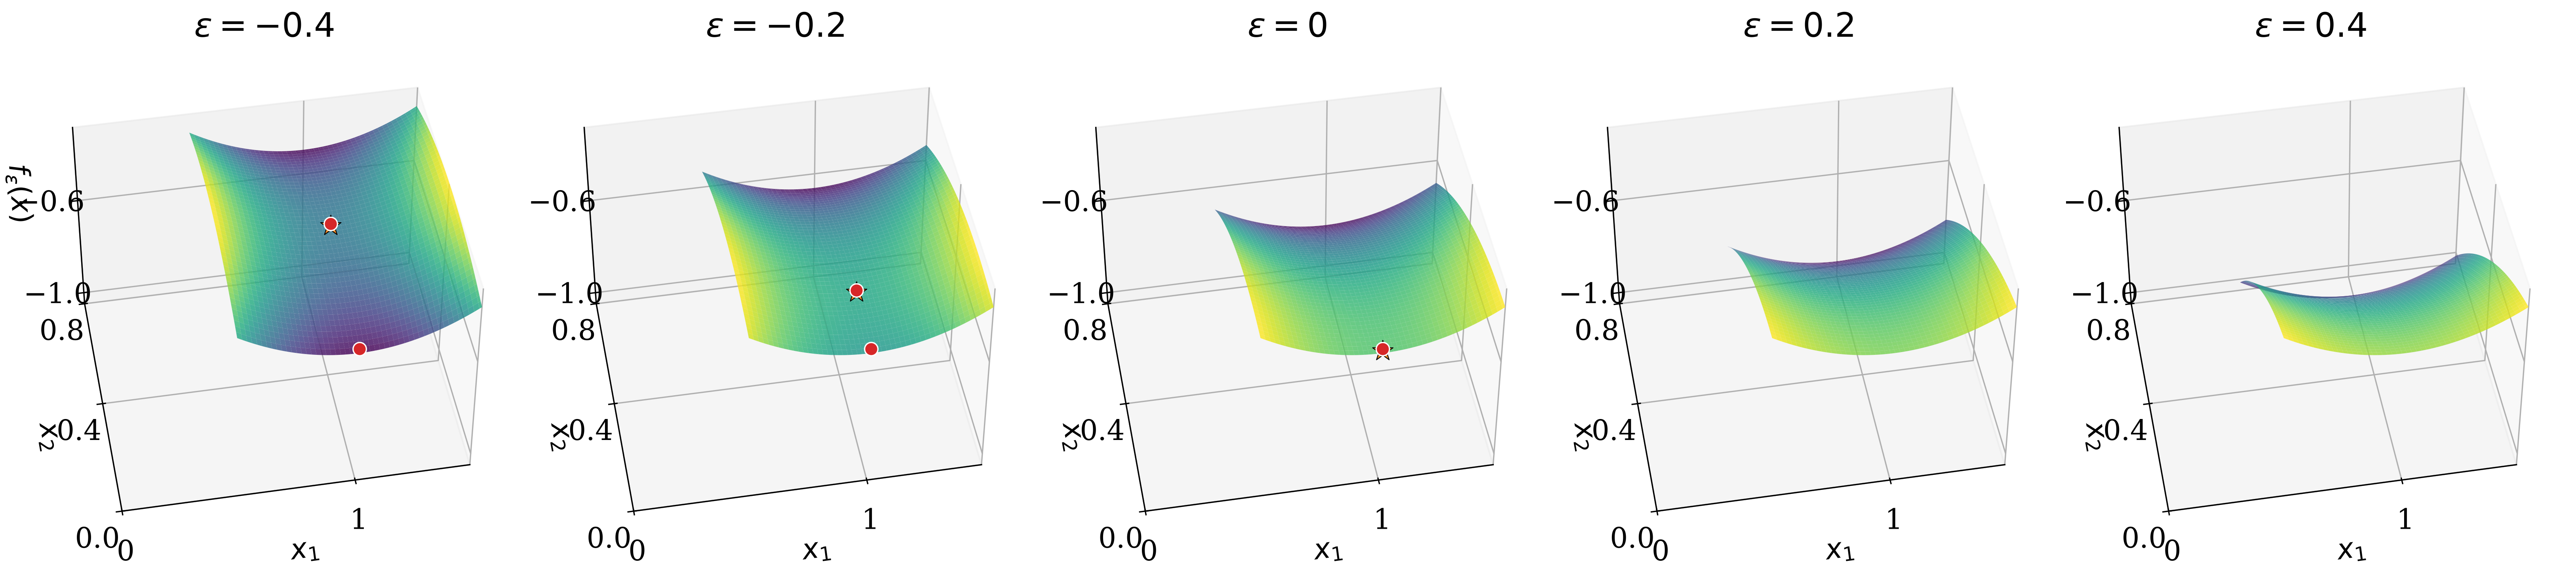
\includegraphics[width=\columnwidth]{optimization_surface_example.png}
        \caption{先ほどの例で、quiverで示した矢印が、$-\nabla f$ となるような $f$ のプロット。}
    \end{figure}
}

\bookBox{証明}{
    証明ではnormal mapのみについて証明する。natural mapも同様。
    解 $x^*$ に対応するnormal mapでの零点を $z^*$ とする。
    $x \mapsto F(x)$ と $x\mapsto x-z^*$ を結ぶホモトピー
    \[
        F_t(x)=tF(x)+(1-t)(x-z^*)
    \]
    を作る。
    このホモトピーに対応するnormal map上において、degree theoryを適用する。
    なんやかんやすると、そのホモトピーの途中でもし零点を持つならば(degreeが変わりうるのならば)、正規化した解差の極限から非零臨界方向 $v$ が得られ、式(5.1.4) に反する(詳細は理解せず)。ゆえに次数は恒等写像の場合と同じ $1$ である。
}

\bookBox{補題5.1.7:解の移動量の制御}{
    式(5.1.4)を満たすのならば、
    $x^*$ に解が存在しない $x^*$ の近傍 $N$ に対してある $c>0$ が存在し、任意の $q \in \mathbb{R}^n$ に対して、
    \[
        \sup\{\norm{x-x^*}:x\in\operatorname{SOL}(K,q+F)\cap\overline N\}
        \le c\norm{q}
    \]
    となる。(証明は背理法で行われる。完全には理解せず。)

    これと局所可解性を合わせると、ある $c,\varepsilon>0$ が存在して、
    \[
        \gamma\coloneqq\sup_{x\in K\cap\overline N}\norm{G(x)-F(x)}<\varepsilon
    \]
    ならば $\operatorname{SOL}(K,G)\cap N\ne\varnothing$ かつ
    \[
        \sup_{x\in\operatorname{SOL}(K,G)\cap\overline N}\norm{x-x^*}
        \le c\gamma.                                                        \tag{5.1.5}
    \]
    パラメータ付きの場合には $\gamma\le L\norm{p-p^*}$ より、局所解写像について上側 Lipschitz 性が得られる。
}

\newpage

\bookBox{5.2節}{
    $K=\mathbb R^n$ とすれば VI は方程式 $H(x)=0$ になる。
}

\myBox{解釈}{
    今までは$K$の境界付近での議論を例にとることが多かったが、ここではそうではなくて、$K$の内点における議論のようなことをしていると解釈できる。
}

\bookBox{5.2 B微分可能方程式:半安定性と安定性}{
    $H$ が零点 $x$ で B微分可能なとき、
    次の三条件は同値である（補題5.2.1）:
    \begin{enumerate}[label=(\alph*)]
        \item $H'(x;v)=0$ ならば $v=0$;
        \item ある $c'>0$ により $\norm{v} \le c'\norm{H'(x;v)}$ が全ての $v$ で成り立つ;
        \item ある近傍 $N$ と $c>0$ により $\norm{y-x}\le c\norm{H(y)}$ が全ての $y\in N$ で成り立つ。
    \end{enumerate}
    とくにこれらは $x$ の孤立性を含意する。さらに
    $\Gamma(y)=H'(x;y-x)$ とおいて $\operatorname{ind}(\Gamma,x)\ne0$ なら、
    十分小さい一様摂動 $G$ は $x$ の近傍に零点をもつ（補題5.2.2）。
}

\myBox{勾配による解釈}{
    \begin{enumerate}[label=(\alph*)]
        \item ヘッセ行列の全ての固有値が非零であることを意味している。
        \item ヘッセ行列の固有値の絶対値の最小値が、$1/c'$以上である
        \item 零点から少しだけ動かすと、動かした先の勾配のノルムの絶対値がある程度以上正になっている
    \end{enumerate}
    最後だけややトリッキーだが、直感的にはいずれも自明。
}

\bookBox{定義5.2.3 半安定と安定}{
    孤立零点 $x$ の性質について、次のように定義する。
    \begin{itemize}
        \item \textbf{半安定}:小さい任意の摂動 $G$ の近傍零点 $x'$ が
              $\norm{x'-x}\le c\norm{H(x')}$ を満たす。ただし摂動後の零点の存在は要求しない。
        \item \textbf{安定}:上の誤差評価に加えて、全ての十分小さい摂動 $G$ が近傍に零点をもつ。
    \end{itemize}
    よって $H'(x;\cdot)$ の零点が原点だけなら半安定であり、さらに指数が非零なら安定である（定理5.2.4）。
    これらは局所概念であり、十分小さな近傍だけを考えればよい。
}

\myBox{半安定だが安定でない点とは?}{
    これが個人的にめちゃくちゃ非自明(これの理解につまりすぎて以降を読むのを諦めました)。\\
    鞍点の例が実際に半安定だが安定ではないのか? と思っていたが、恐らくこれは安定。摂動に対しても、安定的に鞍点が作られる。\\
    関数の勾配的な解釈においては、3次関数のような場合を考えると、確かに摂動に対して零点が存在しなくなるような例が作れることが分かる。
}

\end{document}
